\FloatBarrier
% Please add the following required packages to your document preamble:
% \usepackage{graphicx}
\begin{table}[h!]
\footnotesize
\centering
\caption{Hyperparameters for each of the various models trained on the AudioSet - Speech Vs. Non-Speech dataset.}
\label{tab:sns_hyp}
\begin{tabular}{lccc}
\hline
\multicolumn{4}{c}{\textbf{AudioSet Hyperparameters}}            \\ \hline
\multicolumn{1}{l|}{\textbf{Parameter}}     & \textbf{MM}        & \textbf{C-MAM Audio} & \textbf{C-MAM Video} \\ \hline
\multicolumn{1}{l|}{\textbf{Epochs}}        & 20   & 50   & 50   \\
\multicolumn{1}{l|}{\textbf{Loss Function}} & BinaryCrossEntropy & MSE                  & MSE                  \\
\multicolumn{1}{l|}{\textbf{Optimizer}}     & Adam & Adam & Adam \\
\multicolumn{1}{l|}{\textbf{Learning Rate}} & 5e-4 & 1e-4 & 1e-4 \\
\multicolumn{1}{l|}{\textbf{Weight Decay}}  & 4e-5 & 4e-5 & 5e-5 \\
\multicolumn{1}{l|}{\textbf{Batch Size}}    & 128  & 128  & 128  \\ \hline
\end{tabular}%
\end{table}


\begin{table}[h!]
    \footnotesize
    \centering
    \caption{Architectures for each model trained on the AudioSet -  Speech Vs. Non-Speech dataset.}
    \label{tab:audioset}
    \begin{minipage}[t]{0.4\textwidth}
        \centering
        \vspace{0pt} % Align tops
        
        \begin{tabular}{clllllllllll}
            \hline
            \multicolumn{12}{c}{\textbf{AudioSet Multimodal Model}}                  \\ \hline
            \multicolumn{6}{c|}{ConvBlock - (1, 16, 16, 32)}   & \multicolumn{6}{l}{\multirow{7}{*}{}} \\ \cline{1-6}
            \multicolumn{6}{c|}{Dropout - (0.55)}     & \multicolumn{6}{l}{}                  \\ \cline{1-6}
            \multicolumn{6}{c|}{AvgPool2d - (4, 4)}   & \multicolumn{6}{l}{}                  \\ \cline{1-6}
            \multicolumn{6}{c|}{Linear - (17472, 64)}      & \multicolumn{6}{l}{}                  \\ \cline{1-6}
            \multicolumn{6}{c|}{BatchNorm1d - (64)} & \multicolumn{6}{l}{}                  \\ \cline{1-6}
            \multicolumn{6}{c|}{ReLU}        & \multicolumn{6}{l}{}                  \\ \cline{1-6}
            \multicolumn{6}{c|}{Linear - (64, 16)}      & \multicolumn{6}{l}{}                  \\ \hline
            \multicolumn{6}{c|}{BatchNorm1d - (64)} & \multicolumn{6}{c}{Linear - (400, 256)}            \\ \hline
            \multicolumn{12}{c}{Linear - (64 + 256, 128)}                                              \\ \hline
            \multicolumn{12}{c}{ReLU}                                                \\ \hline
            \multicolumn{12}{c}{Dropout - (0.5)}                                             \\ \hline
            \multicolumn{12}{c}{Linear - (128, 64)}                                              \\ \hline
            \multicolumn{12}{c}{ReLU}                                                \\ \hline
            \multicolumn{12}{c}{Dropout - (0.5)}                                             \\ \hline
            \multicolumn{12}{c}{Linear - (64, 1)}                                              \\ \hline
            \end{tabular}
    \end{minipage}%
    \hfill
    \begin{minipage}[t]{0.24\textwidth}
        \centering
        \vspace{0pt} % Align tops
        \begin{tabular}{|clllll|}
            \hline
            \multicolumn{6}{c}{\textbf{AudioSet Audio C-MAM}} \\ \hline
            \multicolumn{6}{c}{Linear - (400, 256)}                            \\ \hline
            \multicolumn{6}{c}{Linear - (256, 64)}                            \\ \hline
            \multicolumn{6}{c}{BatchNorm1d - (64)}                       \\ \hline
            \multicolumn{6}{c}{ReLU}                              \\ \hline
            \multicolumn{6}{c}{Dropout - (0.5)}                           \\ \hline
            \multicolumn{6}{c}{Linear - (64, 16)}                            \\ \hline
            \end{tabular}
    \end{minipage}%
    \hfill
    \begin{minipage}[t]{0.24\textwidth}
    \centering
    \vspace{0pt} % Align tops
        \begin{tabular}{|clllll|}
        \hline
        \multicolumn{6}{c}{\textbf{AudioSet Video C-MAM}} \\ \hline
        \multicolumn{6}{c}{ConvBlock - (1, 16, 16, 32)}                     \\ \hline
        \multicolumn{6}{c}{Dropout - (0.55)}                       \\ \hline
        \multicolumn{6}{c}{AvgPool2d - (4, 4)}                     \\ \hline
        \multicolumn{6}{c}{Linear - (17472, 64)}                        \\ \hline
        \multicolumn{6}{c}{BatchNorm1d - (64)}                   \\ \hline
        \multicolumn{6}{c}{ReLU}                          \\ \hline
        \multicolumn{6}{c}{Linear - (64, 16)}                        \\ \hline
        \multicolumn{6}{c}{Linear - (16, 64)}                        \\ \hline
        \multicolumn{6}{c}{BatchNorm1d - (64)}                   \\ \hline
        \multicolumn{6}{c}{ReLU}                          \\ \hline
        \multicolumn{6}{c}{Dropout - (0.5) }                       \\ \hline
        \multicolumn{6}{c}{Linear - (64, 256)}                        \\ \hline
        \end{tabular}
    \end{minipage}
\end{table}


% \subsection{AudioSet - Speech vs Non-Speech All Results}
% \label{sec:app_sns_full_results}
% \begin{figure}[h!]
%     \centering
%     \begin{minipage}{0.45\textwidth}
%         \centering
%         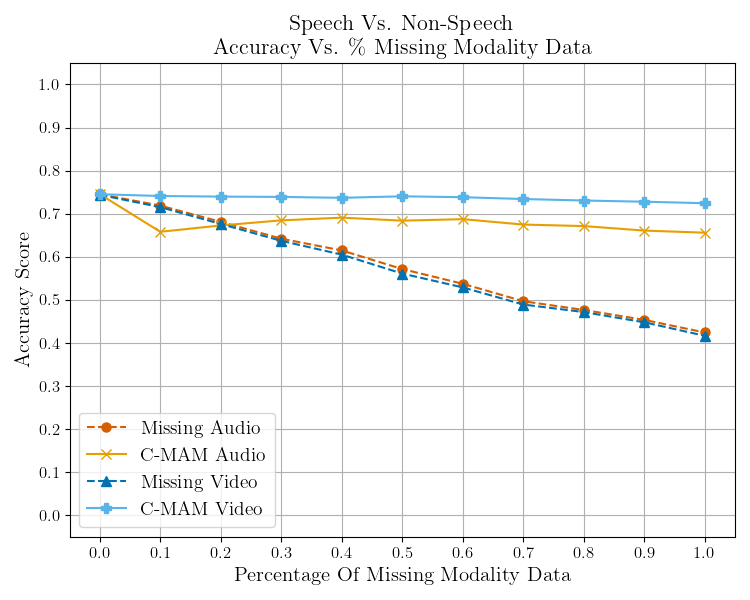
\includegraphics[width=0.9\textwidth]{imgs/sns_results/accuracy.png} % first figure itself
%     \end{minipage}\hfill
%     % Remove or comment out this line
%     \begin{minipage}{0.45\textwidth}
%         \centering
%         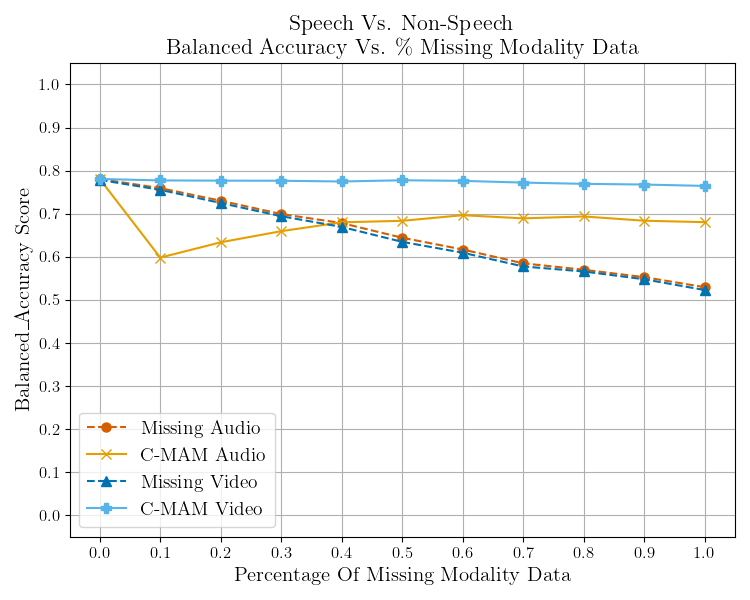
\includegraphics[width=0.9\textwidth]{imgs/sns_results/balanced_accuracy.png} % second figure itself
%     \end{minipage}
%         \begin{minipage}{0.45\textwidth}
%         \centering
%         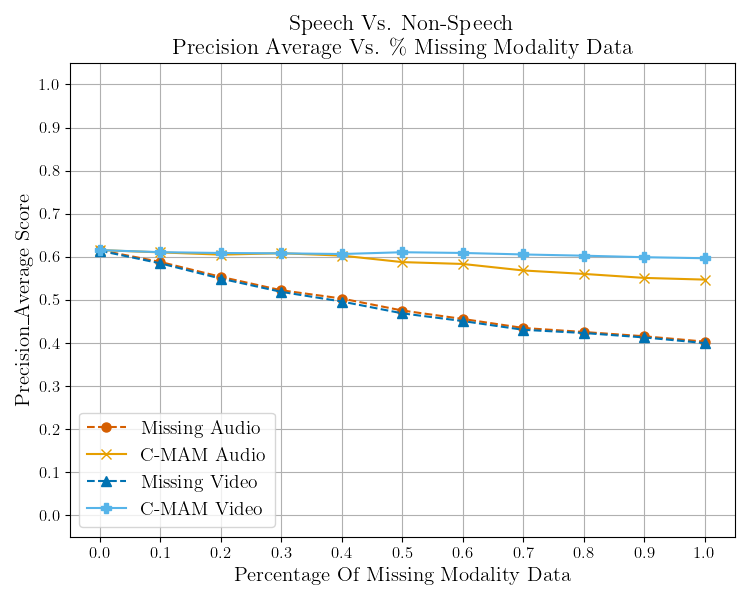
\includegraphics[width=0.9\textwidth]{imgs/sns_results/precision_average.png} % first figure itself
%     \end{minipage}\hfill
%     % Remove or comment out this line
%     \begin{minipage}{0.45\textwidth}
%         \centering
%         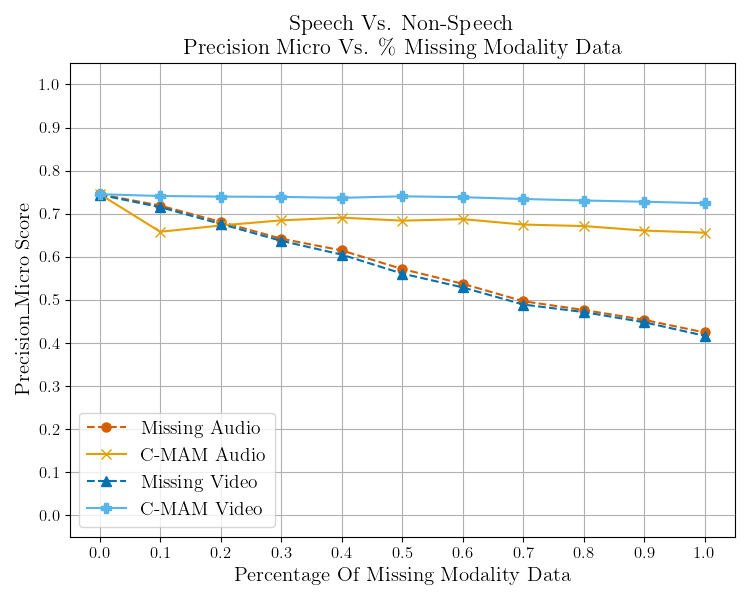
\includegraphics[width=0.9\textwidth]{imgs/sns_results/precision_micro.png} % second figure itself
%     \end{minipage}
%             \begin{minipage}{0.45\textwidth}
%         \centering
%         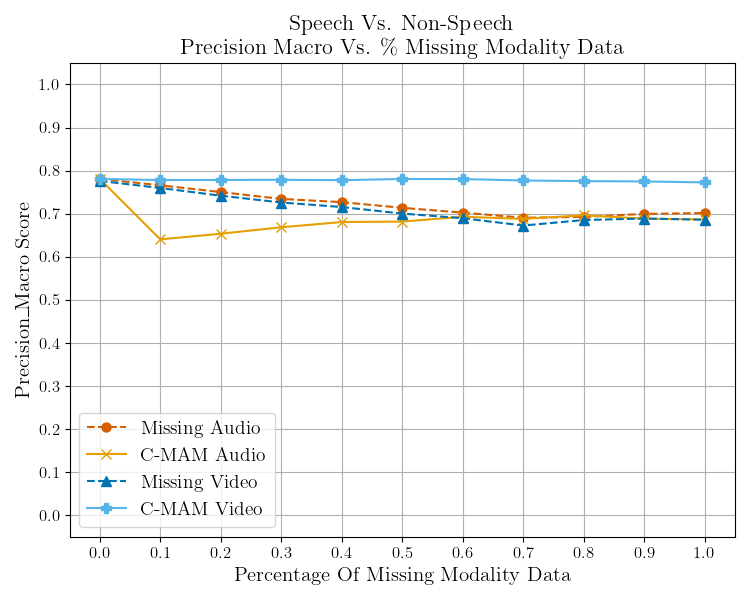
\includegraphics[width=0.9\textwidth]{imgs/sns_results/precision_macro.png} % first figure itself
%     \end{minipage}\hfill
%     % Remove or comment out this line
%     \begin{minipage}{0.45\textwidth}
%         \centering
%         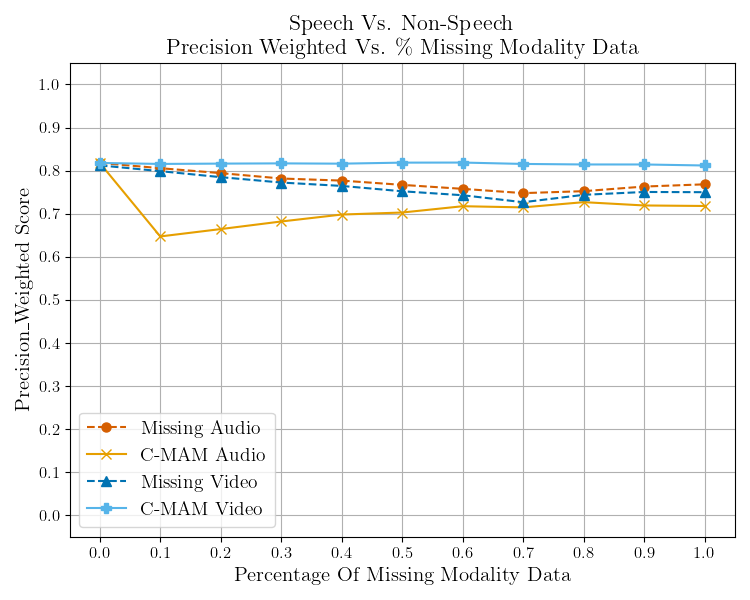
\includegraphics[width=0.9\textwidth]{imgs/sns_results/precision_weighted.png} % second figure itself
%     \end{minipage}

%             \begin{minipage}{0.45\textwidth}
%         \centering
%         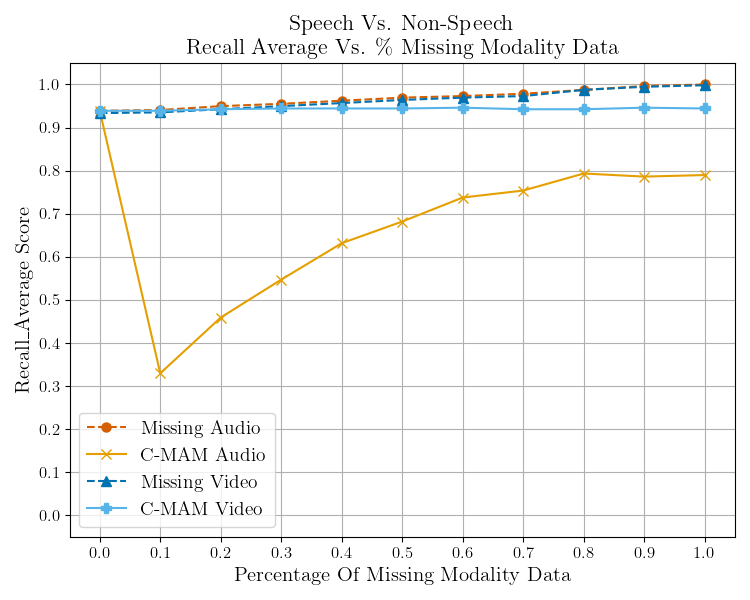
\includegraphics[width=0.9\textwidth]{imgs/sns_results/recall_average.png} % first figure itself
%     \end{minipage}\hfill
%     % Remove or comment out this line
%     \begin{minipage}{0.45\textwidth}
%         \centering
%         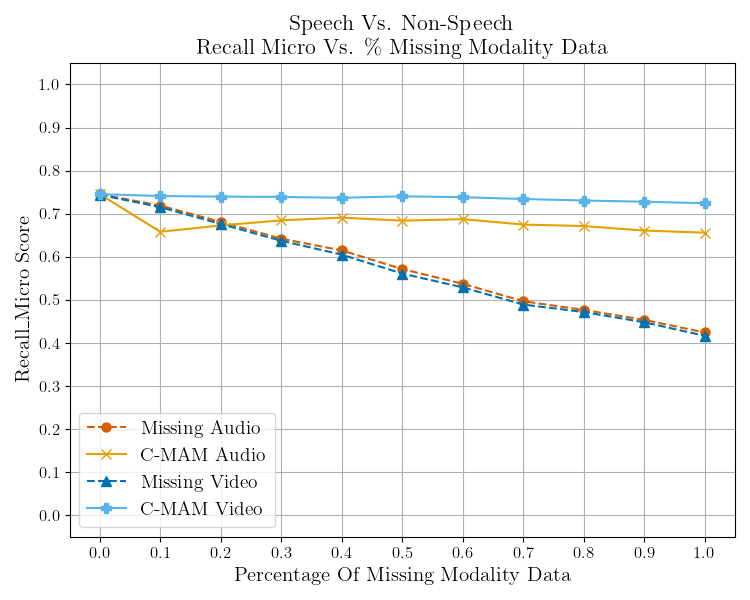
\includegraphics[width=0.9\textwidth]{imgs/sns_results/recall_micro.png} % second figure itself
%     \end{minipage}
% \end{figure}

% \begin{figure} \ContinuedFloat
%     \begin{minipage}{0.45\textwidth}
%         \centering
%         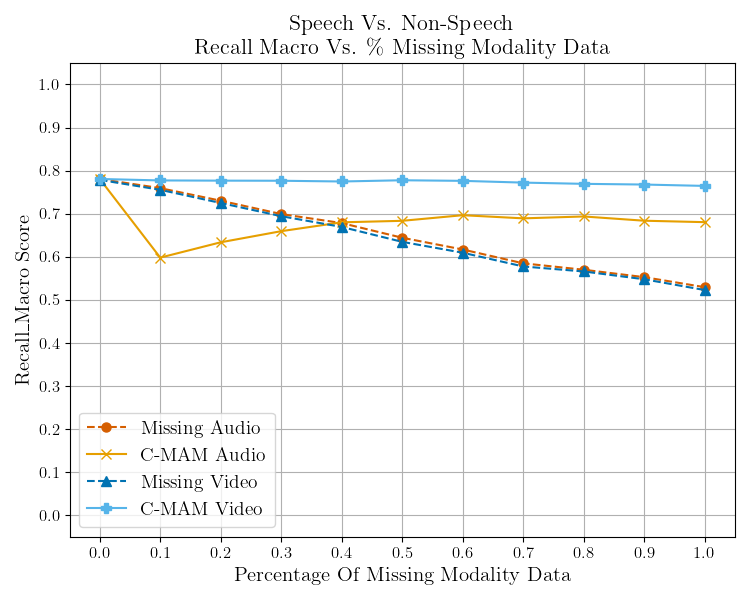
\includegraphics[width=0.9\textwidth]{imgs/sns_results/recall_macro.png} % first figure itself
%     \end{minipage}  
%     % Remove or comment out this line
%     \begin{minipage}{0.45\textwidth}
%         \centering
%         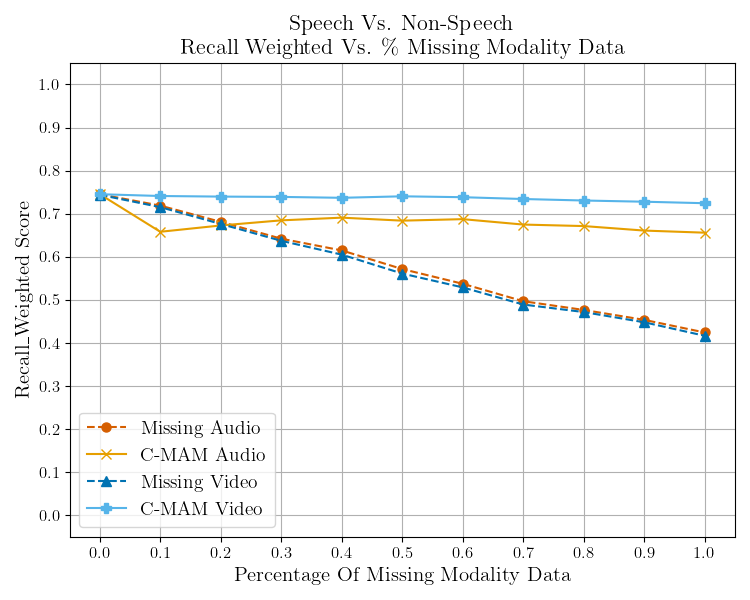
\includegraphics[width=0.9\textwidth]{imgs/sns_results/recall_weighted.png} % second figure itself
%     \end{minipage} 
%     \begin{minipage}{0.45\textwidth}
%         \centering
%         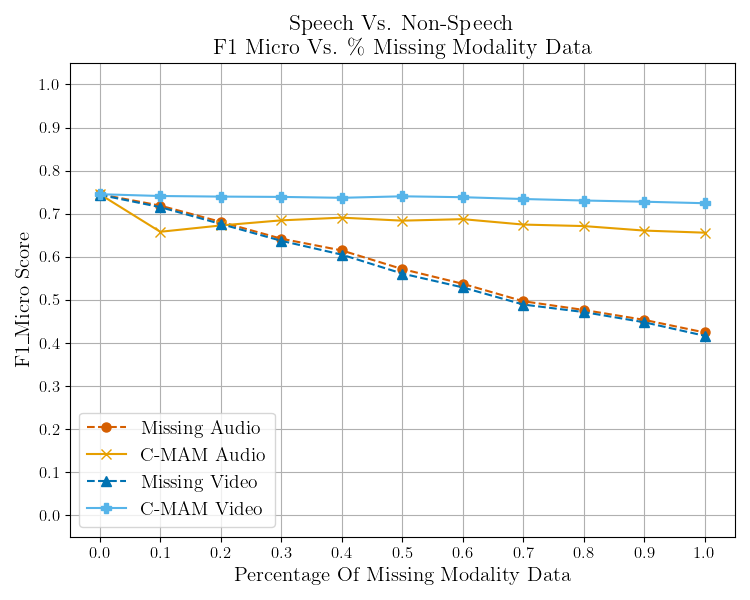
\includegraphics[width=0.9\textwidth]{imgs/sns_results/f1_micro.png} % second figure itself
%     \end{minipage} \hfill
%     \begin{minipage}{0.45\textwidth}
%         \centering
%         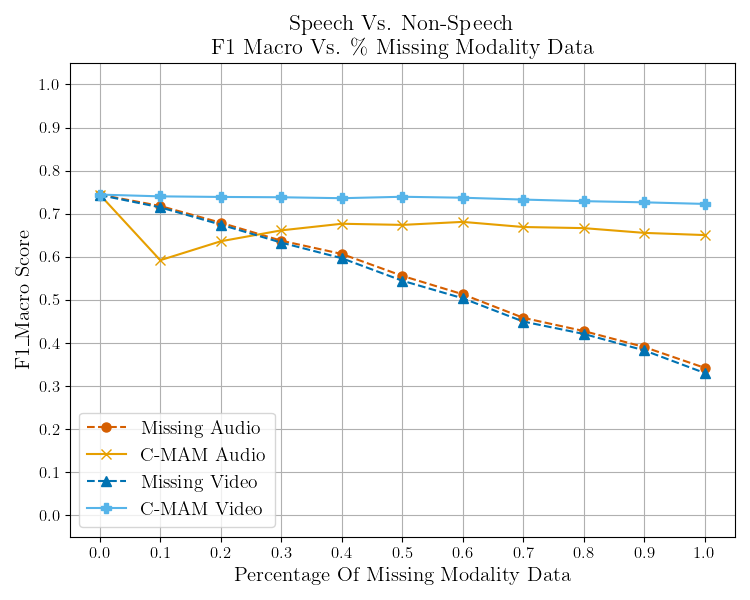
\includegraphics[width=0.9\textwidth]{imgs/sns_results/f1_macro.png} % first figure itself
%     \end{minipage} 
%     % Remove or comment out this line
%     \begin{minipage}{0.45\textwidth}
%         \centering
%         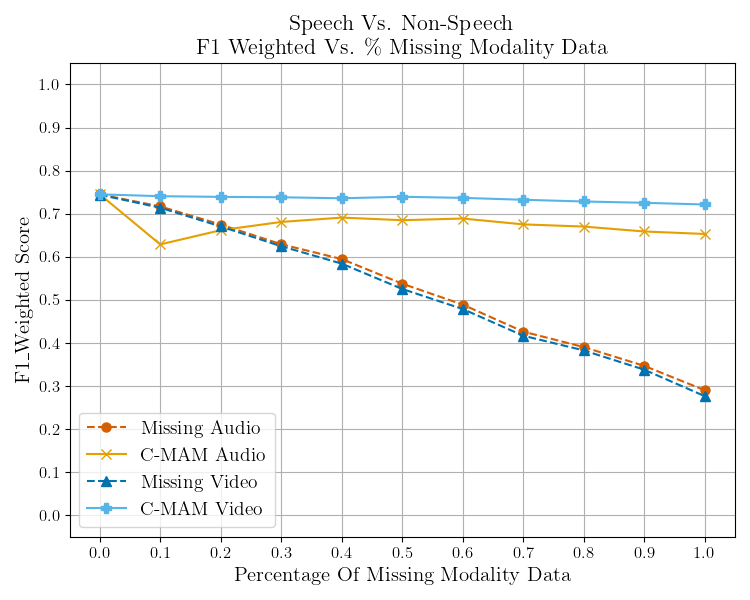
\includegraphics[width=0.9\textwidth]{imgs/sns_results/f1_weighted.png} % second figure itself
%     \end{minipage}
% \end{figure}
% \FloatBarrier
% \newpage